\chapter{जंतु क्या खाते हैं}\label{ch:g2:what-animals-eat}

मैदान का ख़रगोश दिन भर घास कुतरता रहता है। शाम को उसी मैदान से गुज़रने
वाली लोमड़ी को घास में कोई दिलचस्पी नहीं --- उसकी दिलचस्पी ख़रगोश में
है। और कलचिड़ी सुबह केंचुए लेती है और दोपहर बाद चेरियाँ। हर \omterm{def:g1:animals-around-us:animal}{जंतु} को
खाना ही पड़ता है, पर हर \omterm{def:g1:animals-around-us:animal}{जंतु} एक ही चीज़ें नहीं खाता।

\section{खाने वालों के तीन प्रकार}

\begin{definition}[शाकाहारी, मांसाहारी, सर्वाहारी]\label{def:g2:what-animals-eat:kinds}
\omterm{def:g1:animals-around-us:animal}{जंतुओं} को इस आधार पर छाँटा जाता है कि वे क्या खाते हैं:
\begin{itemize}
  \item \emph{शाकाहारी}\index{शाकाहारी} \omterm{def:g1:plants-around-us:plant}{पौधे} खाता है: घास, \omterm{def:g1:plants-around-us:parts}{पत्तियाँ},
        \omterm{def:g2:from-seed-to-plant:seed}{बीज}, फल --- ख़रगोश, गाय, घोंघा;
  \item \emph{मांसाहारी}\index{मांसाहारी} दूसरे \omterm{def:g1:animals-around-us:animal}{जंतुओं} को खाता है:
        लोमड़ी, बिल्ली, गुबरैला (जो नन्हे पौध-चीलरों का शिकार करता
        है);
  \item \emph{सर्वाहारी}\index{सर्वाहारी} \omterm{def:g1:plants-around-us:plant}{पौधे} और \omterm{def:g1:animals-around-us:animal}{जंतु} दोनों खाता है:
        कलचिड़ी, जंगली सूअर --- और मनुष्य।
\end{itemize}
\end{definition}

\begin{example}[एक मैदान, तीन मेनू]\label{ex:g2:what-animals-eat:meadow}
गर्मियों के एक मैदान में: ख़रगोश घास कुतरता है (\omterm{def:g2:what-animals-eat:kinds}{शाकाहारी}); लोमड़ी
ख़रगोश का शिकार करती है (\omterm{def:g2:what-animals-eat:kinds}{मांसाहारी}); कलचिड़ी अभी एक केंचुआ लेती है,
थोड़ी देर बाद एक चेरी (\omterm{def:g2:what-animals-eat:kinds}{सर्वाहारी})। तीन पड़ोसी, तीन मेनू --- और ध्यान
दो कि लोमड़ी के खाने ने पहले घास खाई थी।
\end{example}

\begin{omfigure}
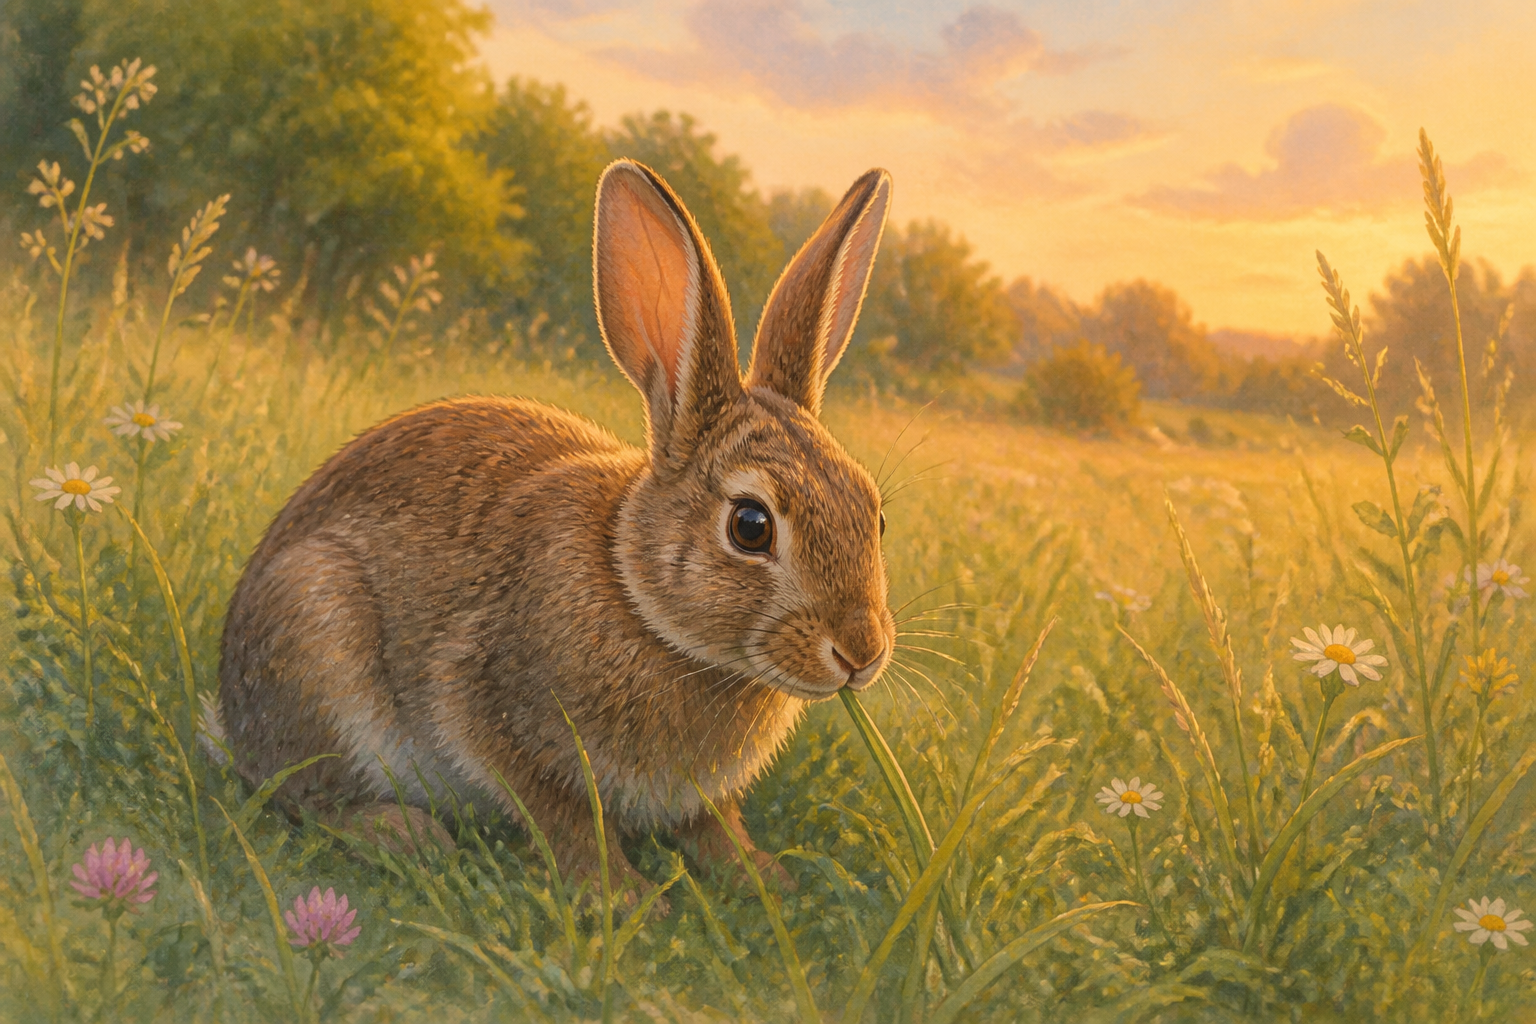
\includegraphics[width=0.6\linewidth]{images/book1/ai/g2-eat-rabbit.png}

{\small एक \omterm{def:g2:what-animals-eat:kinds}{शाकाहारी} काम पर: ख़रगोश और मैदान, तिनका दर तिनका।}
\end{omfigure}

\begin{remark}[मांसाहारी खलनायक नहीं होते]\label{rem:g2:what-animals-eat:fox}
ख़रगोश खाने से लोमड़ी ``दुष्ट'' नहीं हो जाती: शिकार करना बस \omterm{def:g2:what-animals-eat:kinds}{मांसाहारी}
के खाने का ढंग है --- उतना ही स्वाभाविक जितना ख़रगोश का कुतरना।
प्रकृति में खाना और खाया जाना जीवन के चलने का हिस्सा हैं; आगे का एक
अध्याय इन सारे भोजनों को आहार शृंखलाओं में पिरो देगा।
\end{remark}

\section{जंतु के शरीर से उसका मेनू पढ़ना}

\begin{proposition}[शरीर मेनू से मेल खाते हैं]\label{prop:g2:what-animals-eat:match}
\omterm{def:g1:animals-around-us:animal}{जंतु} का शरीर उसके भोजन के सुराग़ लिए रहता है:
\begin{itemize}
  \item ख़रगोश और गाय जैसे \omterm{def:g2:what-animals-eat:kinds}{शाकाहारियों} के गाल वाले दाँत बड़े और चपटे
        होते हैं, जो \omterm{def:g1:plants-around-us:plant}{पौधों} को पीसते हैं, और वे घंटों खाते रहते हैं;
  \item बिल्ली और लोमड़ी जैसे \omterm{def:g2:what-animals-eat:kinds}{मांसाहारियों} के दाँत नुकीले होते हैं,
        जो शिकार को दबोचते हैं, पंजे तेज़ होते हैं, और \omterm{def:g1:the-five-senses:sense}{आँखें} शिकार के
        लिए आगे की ओर देखती हैं;
  \item पक्षियों में यह चोंच से पता चलता है: \omterm{def:g2:from-seed-to-plant:seed}{बीज} तोड़ने के लिए छोटी
        और मोटी (गौरैया), माँस फाड़ने के लिए मुड़ी और अँकुड़ीदार
        (उकाब), छाल से कीट निकालने के लिए लंबी और पतली।
\end{itemize}
\end{proposition}
\admitted

\begin{omfigure}
\begin{minipage}[t]{0.31\linewidth}\centering
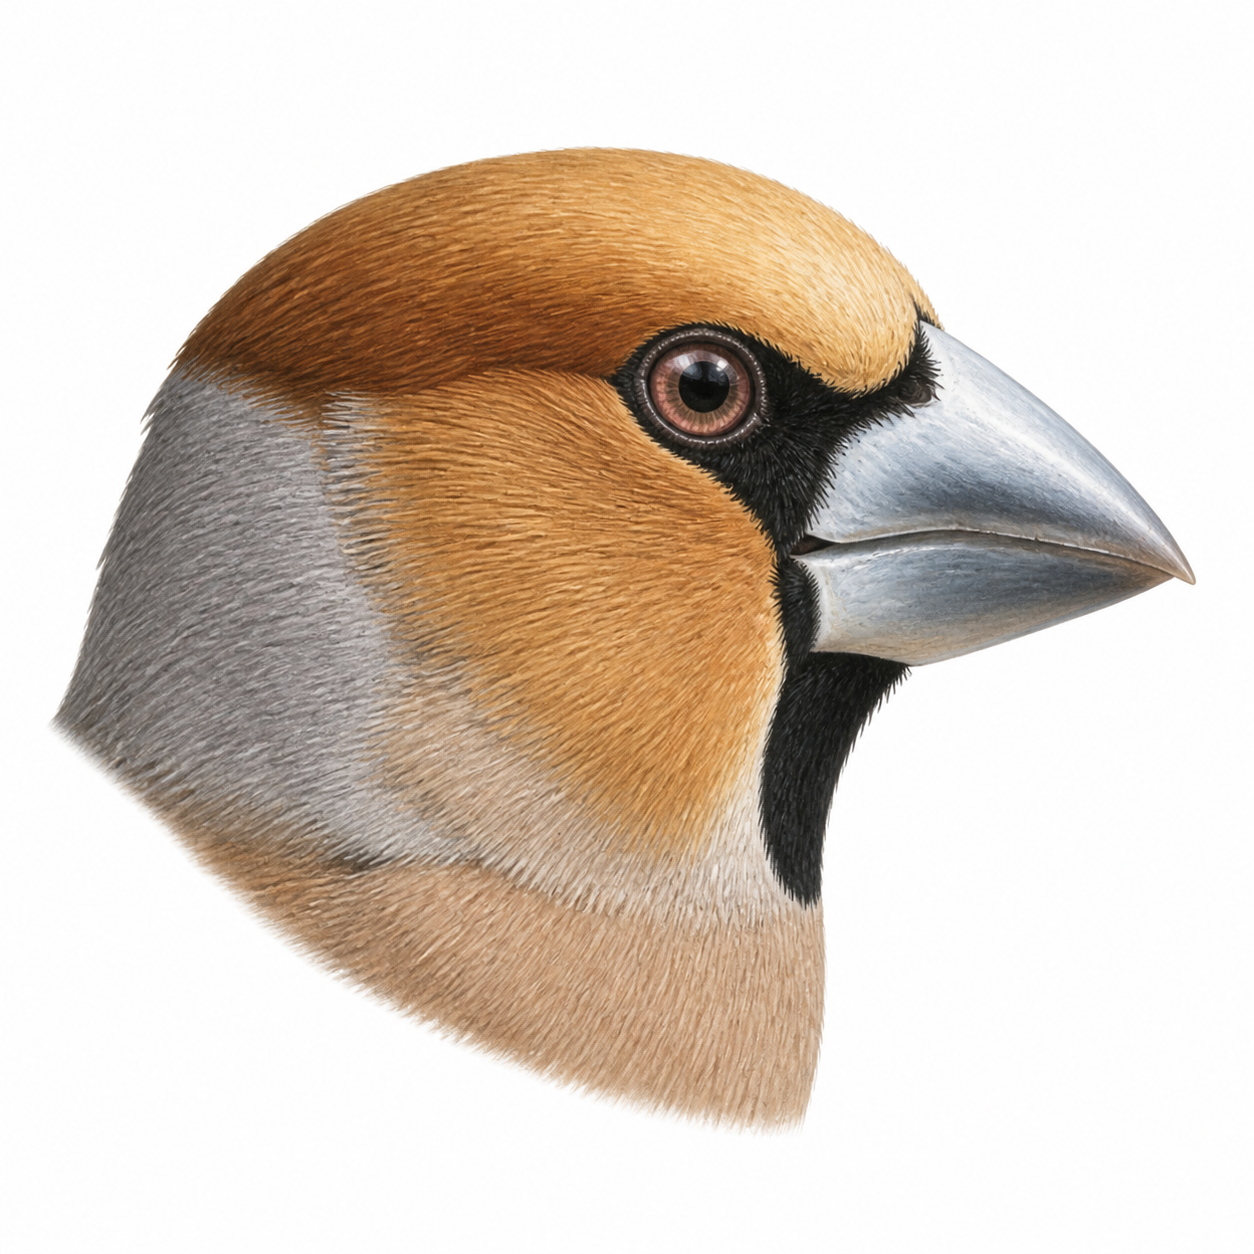
\includegraphics[width=\linewidth]{images/book1/ai/fig-beak-seed.png}

{\small छोटी मोटी चोंच:\\ \omterm{def:g2:from-seed-to-plant:seed}{बीज} तोड़ती है}
\end{minipage}\hfill
\begin{minipage}[t]{0.31\linewidth}\centering
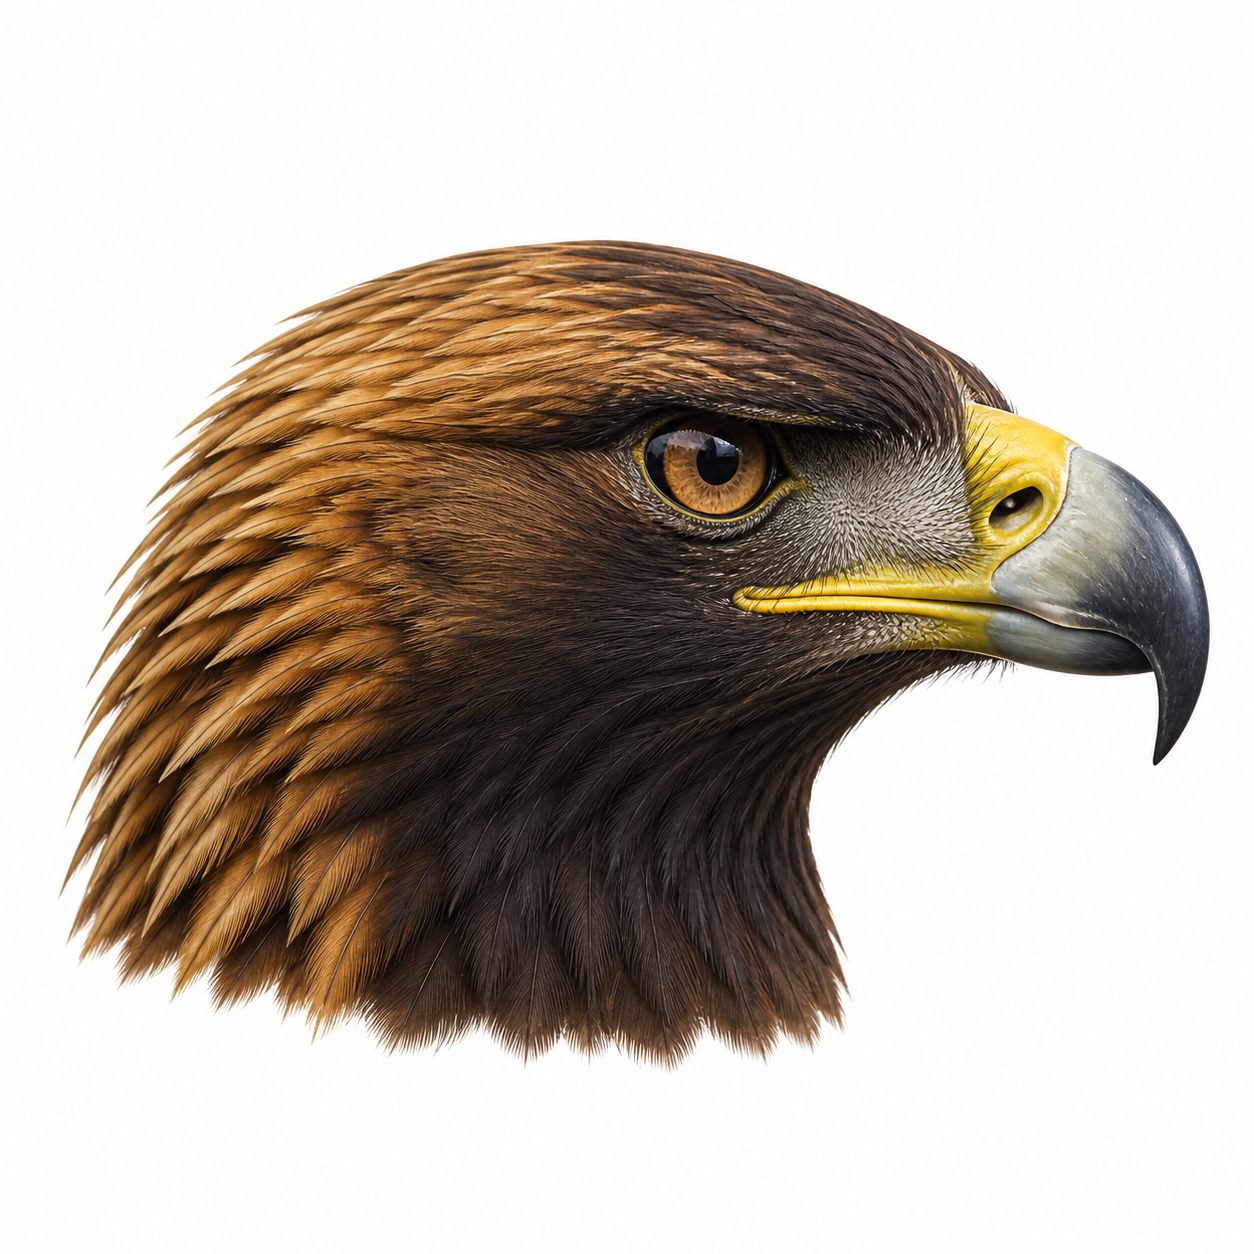
\includegraphics[width=\linewidth]{images/book1/ai/fig-beak-hook.png}

{\small अँकुड़ीदार चोंच:\\ माँस फाड़ती है}
\end{minipage}\hfill
\begin{minipage}[t]{0.31\linewidth}\centering
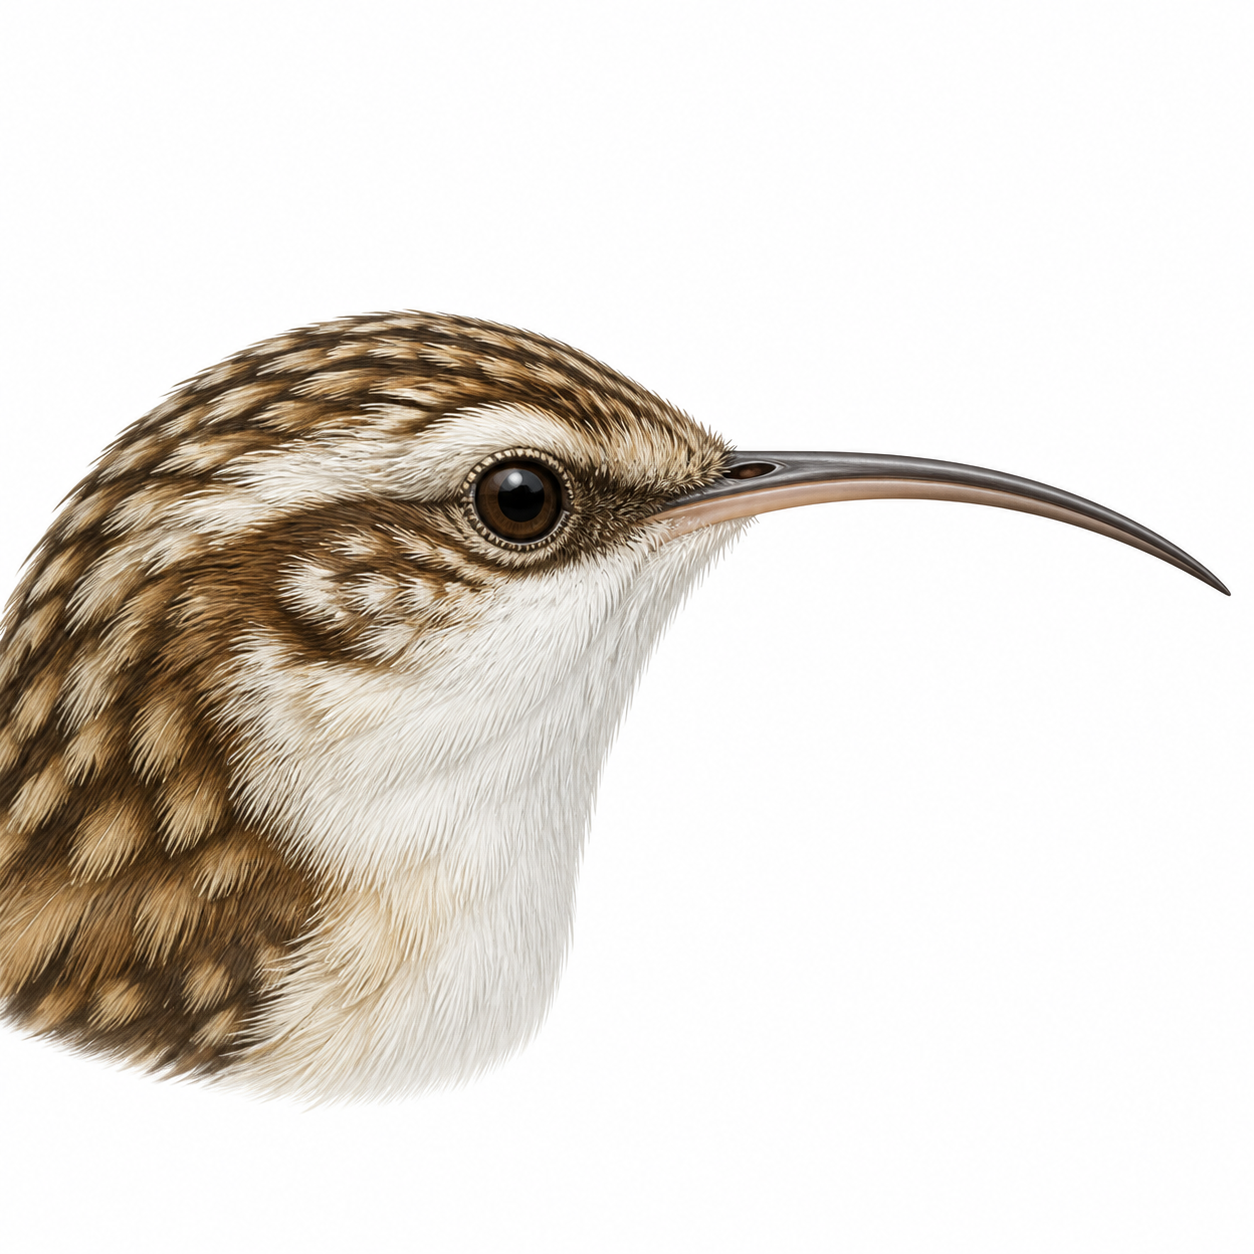
\includegraphics[width=\linewidth]{images/book1/ai/fig-beak-thin.png}

{\small लंबी पतली चोंच:\\ कीट निकालती है}
\end{minipage}

\medskip
{\small तीन चोंचें, तीन मेनू: पक्षी की चोंच वह औज़ार है जिसे उसके
भोजन ने गढ़ा है।}
\end{omfigure}

\begin{example}[बिल्ली के दाँत]\label{ex:g2:what-animals-eat:cat}
बिल्ली को जम्हाई लेते देखो: उसके मुँह के अगले कोनों पर लंबे नुकीले
दाँत। ये दबोचने वाले दाँत हैं --- \omterm{def:g2:what-animals-eat:kinds}{मांसाहारी} का साज़-सामान। गाय जम्हाई
ले तो ऐसा एक भी न दिखे: उसका मुँह घास के लिए चौड़े, चपटे पीसने वालों
से भरा है।
\end{example}

\begin{method}[मेनू का अंदाज़ा लगाना]\label{met:g2:what-animals-eat:guess}
किसी अनजान \omterm{def:g1:animals-around-us:animal}{जंतु} का भोजन बूझने के लिए:
\begin{enumerate}
  \item दाँत या चोंच देखो: चपटे पीसने वाले, नुकीले दबोचने वाले, या
        दोनों?
  \item पंजे और \omterm{def:g1:the-five-senses:sense}{आँखें} देखो: शिकार के औज़ार हैं या नहीं?
  \item हो सके तो उसे खाते हुए देखो --- यही सबसे पक्का सुराग़ है;
  \item फिर उसका नाम दो: \omterm{def:g2:what-animals-eat:kinds}{शाकाहारी}, \omterm{def:g2:what-animals-eat:kinds}{मांसाहारी} या \omterm{def:g2:what-animals-eat:kinds}{सर्वाहारी}।
\end{enumerate}
\end{method}

\section{रोज़-रोज़ पेट भरना}

\begin{proposition}[खाना रोज़ का काम है]\label{prop:g2:what-animals-eat:daily}
भोजन शरीर का ईंधन भी है और उसका बनाने वाला सामान भी, इसलिए \omterm{def:g1:animals-around-us:animal}{जंतुओं} को
बार-बार, दिन दर दिन खाना पड़ता है। इसमें कितना समय लगेगा, यह मेनू पर
निर्भर है: घास हर कौर में थोड़ा ही देती है, इसलिए गाय घंटों चरती है;
माँस भरपूर होता है, इसलिए लोमड़ी एक अच्छा भोजन करके आराम कर सकती है।
\end{proposition}
\admitted

\begin{example}[सर्दी मेनू बदल देती है]\label{ex:g2:what-animals-eat:winter}
भोजन मौसम के साथ बदलता है। कलचिड़ी गर्मियों में केंचुए और कीट खाती है,
पर सर्दियों में, जब ज़मीन सख़्त हो जाती है, वह जामुनों पर आ जाती है।
मुश्किल दिनों में \omterm{def:g2:what-animals-eat:kinds}{सर्वाहारी} का चौड़ा मेनू बड़ी मदद करता है।
\end{example}

\section{अभ्यास}

\begin{exercise}[$\star$]\label{exo:g2:what-animals-eat:1}
इनके लिए शब्द बताओ: \omterm{def:g1:plants-around-us:plant}{पौधे} खाने वाला \omterm{def:g1:animals-around-us:animal}{जंतु}; दूसरे \omterm{def:g1:animals-around-us:animal}{जंतुओं} को खाने वाला
\omterm{def:g1:animals-around-us:animal}{जंतु}; दोनों खाने वाला \omterm{def:g1:animals-around-us:animal}{जंतु}।
\end{exercise}

\begin{exercise}[$\star$]\label{exo:g2:what-animals-eat:2}
\omterm{def:g2:what-animals-eat:kinds}{शाकाहारी}, \omterm{def:g2:what-animals-eat:kinds}{मांसाहारी} या \omterm{def:g2:what-animals-eat:kinds}{सर्वाहारी}: (क) गाय; (ख) लोमड़ी; (ग) कलचिड़ी;
(घ) घोंघा; (ङ) मनुष्य?
\end{exercise}

\begin{exercise}[$\star$]\label{exo:g2:what-animals-eat:3}
\omterm{def:g2:what-animals-eat:kinds}{शाकाहारी} को कौन-से दाँत सबसे ज़्यादा चाहिए: चपटे पीसने वाले, या नुकीले
दबोचने वाले? क्यों?
\end{exercise}

\begin{exercise}[$\star$]\label{exo:g2:what-animals-eat:4}
हर चोंच को एक मेनू से मिलाओ: छोटी और मोटी; मुड़ी और अँकुड़ीदार; लंबी
और पतली।
\end{exercise}

\begin{exercise}[$\star$]\label{exo:g2:what-animals-eat:5}
गुबरैला छोटा है, सुंदर है --- और \omterm{def:g2:what-animals-eat:kinds}{मांसाहारी} है। वह किसका शिकार करता
है?
\end{exercise}

\begin{exercise}[$\star$]\label{exo:g2:what-animals-eat:6}
गाय लोमड़ी से कहीं ज़्यादा घंटे खाने में क्यों बिताती है?
\cref{prop:g2:what-animals-eat:daily} का इस्तेमाल करो।
\end{exercise}

\begin{exercise}[$\star$]\label{exo:g2:what-animals-eat:7}
कलचिड़ी गर्मियों में क्या खाती है, और सर्दियों में? चौड़ा मेनू क्यों
काम आता है?
\end{exercise}

\begin{exercise}[$\star$]\label{exo:g2:what-animals-eat:8}
करके देखो: पार्क में या दाना-घर पर पक्षियों को देखो। लिखो कि हर तरह का
पक्षी क्या लेता है --- \omterm{def:g2:from-seed-to-plant:seed}{बीज}, रोटी, कीट, जामुन --- और उनकी चोंचें देखो।
क्या \cref{prop:g2:what-animals-eat:match} सही उतरता है?
\end{exercise}

\begin{exercise}[$\star\star$]\label{exo:g2:what-animals-eat:9}
एक चिड़ियाघर को पहेली वाला \omterm{def:g1:animals-around-us:animal}{जंतु} मिलता है: नुकीले अगले दाँत, तेज़ पंजे,
आगे की ओर देखती \omterm{def:g1:the-five-senses:sense}{आँखें}। उसका संभावित मेनू क्या है?
\cref{met:g2:what-animals-eat:guess} के कौन-से चरण तुमने इस्तेमाल किए?
\end{exercise}

\begin{exercise}[$\star\star$]\label{exo:g2:what-animals-eat:10}
``घास न हो तो जल्द ही लोमड़ियाँ भी न रहेंगी।'' लोमड़ी घास कभी नहीं
खाती --- फिर भी यह वाक्य सही है।
\cref{ex:g2:what-animals-eat:meadow} के मैदान से समझाओ।
\end{exercise}
